\section{Vector Extentions}

As demonstrated earlier in this report, enhancing data load and store operations contributes to the improvement of a system's memory access latency and overall performance. However, individual computations on this data still occur sequentially. This is where vector extensions prove beneficial. Vector extensions employ Single Instruction, Multiple Data (SIMD) instructions across a vector of data in a single execution step, enabling increased system throughput.


\subsection{ARM Scalable Vector Extention}
\label{label:arm-sve}

The ARM approach to a vector-length-agnostic programming model was the creation of the ARM SVE \cite{arm-paper}. The SVE brings a new architectural state with the inclusion of 32 new scalable vector registers, \textit{Z0 to Z31}, (with a total width ranging from 128 to 2,048 bits depending on the implementation), 32 128-bit wide Advance SIMD registers, \textit{V0 to V31}, allowing for 64-, 32-, 16- and 8-bit scalable containers, 16 scalable predicate registers \textit{P0 to P15} and a set of control registers \textit{ZCR\_EL1 to ZCR\_EL3}.



\subsubsection{Power through Predication}
The ARM SVE solution allows programmers to think at a higher level of abstraction regarding vector length. This is possible through predicate registers that dynamically modify the vector length during execution. It allows the execution of only the lanes that matter, as opposed to the usual SIMD strategy of computing the whole vector and discarding unwanted values through masking.

\begin{figure}[H]
	\begin{center}
 		\includegraphics[width=0.77\linewidth]{images/predicator-example.pdf}
 		\caption{Cycle by cycle example of daxpy with n = 3 and hardware vector lengths of 128- and 256-bit - figure from \cite{arm-paper}}
 		\label{fig:arm-sve-assembly}
	\end{center} 
\end{figure}

Figure \ref{fig:arm-sve-assembly} illustrates a step-by-step example of a Daxpy program for a vector length of 128 and 256 bits. The use of a predicate variable is evident in the 128-bit configuration, with both its values set to true on the first comparison, utilizing the full dimension of the vector. This state of the predicate signifies that the load and computation of values occurs in both positions of the variables \textit{z0, z1, z2}. After the loop iteration,  the variable tracking the number of processed elements is incremented (in this case, by the total of float elements in the vector), and compared with the total number of values to be processed. From this comparison, another predicate is generated, and, since two elements have been processed and the total is three, the new predicate indicates the execution of instructions over only a single entry of \textit{z0, z1, z2} in the next iteration.

Something similar happens in the 256 bits vector configuration how however, the initial comparison generates a predicate with the last position being false. This means the vector won't be utilized in full, but it also indicates that the next predicated instructions to execute should only compute three values.

SVE includes in its extended instruction set a family of \textit{while} instructions that work by populating a new predicate through the use of a scalar counter. The value of this stride can be incremented not only by the value of the total number of elements in the system vector but also through more complex increment functions like incrementing by the number of active lanes, the largest multiple of a data element on a vector, allowing for a powerful data access and manipulation. 

Due to the nature of vector-length-agnostic programming, situations where vector initialization needs to be done can become very difficult. To address this complexity, the presented SVE extension incorporates a set of instructions capable of dynamically generating vector initialization during runtime. This dynamic approach is particularly useful as it adapts to pattern initializations, allowing for flexibility and efficiency in vector initialization processes.

Some examples of specific vector initialization are as follows:
\begin{itemize}
    \item Initializing a vector with a set of indexes that start on 1 and increment by 4 can be achieved using \textit{INDEX Zd.S, \#1, \#4} resulting in \textbf{Zd = [1, 5, 9, 13, 17, 21, 25, 29]} for a vector size of 8 elements.
    \item Initializing a predicate vector that is supposed to contain as many triples of the true value as will fit in the vector:\textit{PTRUE Pd.S, MUL3} will result in  \textbf{Pd = [(T,T,T), (T,T,T), F, F]} for a vector size of 8 elements.
\end{itemize}

\subsubsection{Horizontal Reductions}

Another implemented feature in the ARM SVE is the ability to do operations across lanes of a vector, essentially taking an operation and applying it to every element of the vector, for example, a sum, a bitwise-and, etc. 

Designing a program with these intrinsics in mind allows for better performance. Fig. \ref{fig:horizontal-reductions} shows a comparison between a simple sum of a multiplication of two vectors. In the ARM SVE version without the intrinsic (Fig. \ref{fig:horizontal-reductions}.C) the compiler only manages to exploit the vertical multiplication of vectors a and b, in the intrinsic version (Fig. \ref{fig:horizontal-reductions}.D) a third vector was created to assist the partial sum during each iteration, leaving the reduction of every element for outside the loop with \textit{faddv}.

\begin{figure}[H]
	\begin{center}
 		\includegraphics[width=\linewidth]{images/horizontal-reductions.pdf}
 		\caption{Comparison of assembly code between ARM SVE without and with horizontal intrinsics}
 		\label{fig:horizontal-reductions}
	\end{center} 
\end{figure}

\subsubsection{Handling unknown data vector size}


In earlier instances of ARM SVE examples, predicates have consistently played a crucial role in the loading, storing, and manipulation of data. Nevertheless, scenarios may arise where determining the size of the vector becomes impractical before the data load. 

One approach in such situations could be to load as much data as can fit into a vector. However, this tactic introduces the risk of loading invalid or protected values from memory, potentially triggering a fault.

To avoid the aforementioned problem speculative vectorization can be utilized. SVE incorporates a distinctive predicate that is generated when employing a memory-probing instruction. This instruction essentially examines the memory entries, starting at a base address, and returning a predicate that indicates the regions in memory corresponding to the desired data.

This feature allows for uncounted loops with break conditions to be still manipulated in vectorization form, without the need for size specification. Figure \ref{fig:ffr-example} depicts the utilization of FFR in an uncounted loop on a machine with a vector length set to four and a total data size of six. In the initial iteration, the returned predicate encompasses all entries marked as true, facilitating the loading of a total of four elements. Subsequently, in the second iteration, only the first two elements are identified as true, allowing the program to proceed by loading two values. As the loop progresses to the third iteration, the predicate indicates that no more data is available beyond that point, enabling the program to continue without further loop iterations.

\begin{figure}[H]
	\begin{center}
 		\includegraphics[width=\linewidth]{images/ffr-example copy.pdf}
 		\caption{Simplified example of loop iteration and vector partition with FFR}
 		\label{fig:ffr-example}
	\end{center} 
\end{figure}

Nevertheless, while this feature effectively addresses the challenge posed by an unknown data size, it introduces a potential downside. The increase in the number of instructions within the loop may contribute to heightened pressure on the processor pipeline. This, in turn, could impact the overall efficiency of the vectorization process. Balancing the advantages of dynamic size handling with the potential impact on pipeline performance becomes a crucial consideration in optimizing the execution of SVE instructions.

\subsubsection{Result Analysis}

 The authors of the ARM SVE \cite{arm-paper} conducted a series of workloads in 4 different configurations of the same generic medium-sized out-of-order microprocessor, one without the implementation of SVE, and three implementations with SVE and where the vector size was changed to 128-, 256- or 512-bit vector length.
The overall results of the SVE implementations showed significant speedups, with workloads achieving 3x, 5x and 7.5 for the SVE 128-bit, the SVE 256-bit, and  SVE 512-bit implementation, respectively, when compared with the non-SVE implementation. Some workload tests presented no speedup due to the nature of the test since they do not benefit from vectorization, so performance was very similar between the four configurations.



\subsection{RISC-V Vector Extention}
\label{label:rvv}

The RISC-V Vector Extension, akin to the ARM Scalable Vector Extension (SVE), adopts an Instruction Set Architecture (ISA) that centers around a vector-length-agnostic programming model. RVV operations distinguish themselves solely based on vector-vector and vector-scalar distinctions, considering signed and unsigned types, without specifying element lengths. Consequently, the element length becomes a dynamic parameter in this context. Moreover, RVV allows the utilization of only a segment of a vector register or even a combination of multiple vector registers, introducing the necessity for dynamic parameters in such scenarios.




\subsection{Unlimited Vector Extention with Data Streaming Support}
\label{label:uve}

%Unlimited Vector Extention is a novelty solution that aims to surpass the existing problems of current state-of-the-art solutions of scalable vector extensions through the use of a data streaming engine, combining streaming and SIMD processing, which allows the exploitation of data parallelism.


%The proposed ISA tries to reduce latencies associated with loop control, memory access indexing, and memory access by using new instructions that allow a pre-configuration of the stream and the memory access patterns. 
%This anticipation of the access control allows for accurate and fast prefetching even with multidimensional arrays or indirect memory accesses. 


Unlimited Vector Extension \cite{uve-paper} represents a novelty solution designed to combine faster data access with increased system throughput. Achieving this objective involves the incorporation of a data streaming engine that seamlessly integrates streaming and SIMD processing, thereby enabling the effective utilization of data parallelism.

The envisioned ISA (Instruction Set Architecture) strives to mitigate latencies commonly associated with loop control, memory access indexing, and memory access. This is achieved by introducing novel instructions that facilitate the pre-configuration of the data stream and memory access patterns. The innovative feature of anticipatory access control enables precise and expedited prefetching, even when dealing with multidimensional arrays or indirect memory accesses.


\subsubsection{UVE Features}

\begin{figure}[H]
    \centering
    \includegraphics[width=\linewidth]{images/UVE-Comparison.pdf}
    \caption{A boat.}
    \label{fig:uve-comparison}
\end{figure}

The distinguishability of this solution from  currently developed SIMD solutions (ARM SVE and RISC-V Vector extension (RVV)) comes from features like:
\begin{itemize}
\item[]  \Tbullet{F1}{Decoupled Memory Access} The ability to decouple the memory accesses from the computation part by streaming the data directly to the register, allowing the occurrence of loads/stores in parallel with the data manipulation, thus reducing the memory access latency.
\item[]  \Tbullet{F2}{Indexing-free Loops} Describing the load/store patterns in advance, minimizing the number of instructions related to memory indexing, reducing the pressure on the processor pipeline (see the UVE Fig.\ref{fig:uve-comparison}.D. 
\item[]  \Tbullet{F3}{Simpified Vectorization} The description of memory pattern access allows the Streaming Engine to perform all non-coalesced accesses as linear patterns. This leads to a simplified vectorization since memory is always aligned from the execution pipeline point of view - see Fig. \ref{fig:uve-mem-access}. 
\item[]  \Tbullet{F4}{Implicit Load/Store} Due to the description of the streams in the loop preamble, the indexing instructions can be removed, meaning that all explicit loads and stores are associated with active streams and different vector register.
\end{itemize}

Besides the mentioned features, UVE is also register-size agnostic, similar to SVE and RVV. However, in UVE, there is no need for size control instruction since the Streaming Engine automatically disables all vector elements that fall out of bounds, making the loops simpler with a minimal set of control functions.


\begin{figure}[H]
	\begin{center}
 		\includegraphics[width=\linewidth]{images/UVE-pseudo-code.pdf}
 		\caption{UVE pseudo-code implementation for the computation of the maximum
across the rows on three possible matrices: (A) full matrix, (B) lower triangular
matrix, and (C) full matrix with pointers to an array}
 		\label{fig:uve-mem-access}
	\end{center} 
\end{figure}

\subsubsection{Data Streaming}

A Streaming Engine was also proposed to manage all the stream manipulations.
These streams are defined as a predictable n-dimensional data sequence transferred between memory and the processor.


\begin{equation}
    y(X) = y_{\text{base}} + \sum_{k=0}^{\text{dim}_y} x_k \times S_k
    \quad \text{with } X = \{x_0, \ldots, x_{\text{dim}_y}\} \text{ and } x_k \in [O_k, E_k+O_k]
    \label{eq:mem_model}
\end{equation}

The proposed stream model is defined by Eq. \ref{eq:mem_model} and encoded in a descriptor-based representation, the \textit{Base Stream Descriptor} and possibly modified during run time by \textit{Static Descriptor Modifiers} and/or \textit{Indirect Descriptor Modifiers}.

The \textbf{Base Stream Descriptor} defines a uni-dimensional access pattern. It is represented by three-parameters $\{O, E, S\}$ corresponding to the offset $(O_k)$, size $(E_k)$ and stride $(S_k)$, simple patterns supported by this descriptor can be seen of Figs. \ref{fig:stream-descriptors}.B1, B2 and B3.

\textbf{Static Descriptors Modifiers} are descriptors that can be used in conjunction with parameters of Base Stream Descriptors to modify the access pattern, allowing for loop-conditioned accesses, for example, a lower triangular memory access as depicted in Fig. \ref{fig:stream-descriptors}.B4. This descriptor is represented as the tuple ${T, B, D, E}$ where $T$ corresponds to the target parameter to modify, $B$ is the modification operator (add or sub), $D$ the value applied with the operator, $E$ the number of times the modifier is applied 

The \textbf{Indirect Descriptor Modifier} allows for the content of a stream to modify the values of another stream, creating indirect and indexed scatter-gather patterns. This modifier is represented then by the tuple ${T, B, P}$, with $T$ being the target parameter, $B$ the behavior parameter (supporting adding a dynamic displacement, subtracting a dynamic displacement, and setting a value directly) and $P$ corresponding to the pointer of the origin data stream.

\begin{figure}[H]
	\begin{center}
 		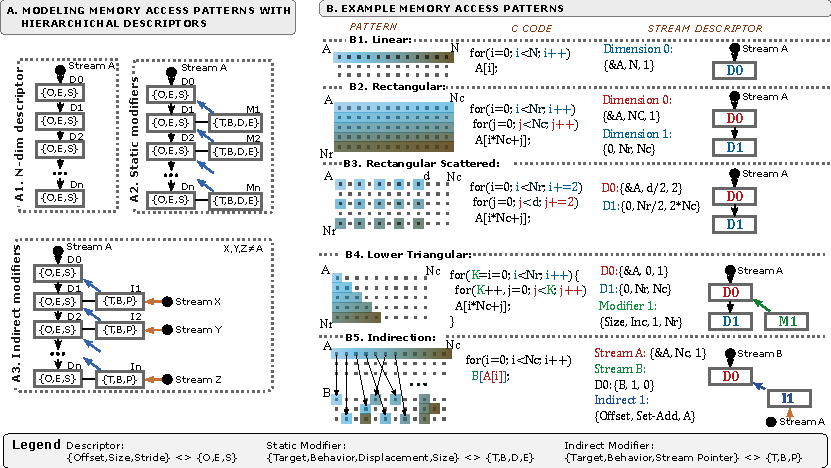
\includegraphics[width=\linewidth]{images/UVE-Descriptors.pdf}
 		\caption{Examples of memory access patterns with UVE descriptors }
 		\label{fig:stream-descriptors}
	\end{center} 
\end{figure}

\subsubsection{Instruction Set}
To utilize the streaming engine, new instructions need to be implemented.

\textbf{Stream configurations} are one of the types of new instructions. As the name implies, these instructions are responsible for encoding the descriptors/modifiers described above, which control the engine's behavior. 

\textbf{Stream control} instructions enable the control of the streams, allowing the momentary stop/restoring of vector registers. This behavior control enables the execution of multiple processes without interfering with stream configurations. 

\textbf{Predication and masking} allow the control of execution of SIMD through the disabling of selected lanes. The proposed UVE provides instructions for predicate configuration based on comparisons and valid vector register elements.

\textbf{Loop control} is assured through three conditional branch formats: predicate-based (condition tested on a specific predicate register), end-of-stream (a condition on the end of a stream), and end-of-dimension (a condition on a stream dimension end).

\textbf{Vector manipulation} instructions allow the common arithmetic, logic, and shift operations to be applied to the vector registers.

\textbf{Advance control} instructions are a subset of specialized instructions that allow the configuration of vector-length and vector-length aligned processing.


\subsubsection{Microachitecture Support}

Besides embedding the streaming engine in the main architecture pipeline, the CPU only needs to be extended with some minor streaming structures. The proposed units to be modified can be seen in Figure \ref{fig:uve-arch}. 

\begin{figure}[H]
	\begin{center}
 		\includegraphics[width=0.77\linewidth]{images/UVE-arch.pdf}
 		\caption{Examples of memory access patterns with UVE descriptors }
 		\label{fig:uve-arch}
	\end{center} 
\end{figure}

The execution unit needs to be modified to understand the instructions proposed in the UVE, in order to utilize vector registers and the corresponding logic, arithmetic, and branch operations.
Renaming of vector registers and streams also needs to be accounted in order to allow speculative stream configurations during the execution of others. The committing stage of the pipeline also needs to be altered to accommodate stream commits.

The included streaming engine has the responsibility of managing all the input and output streams, for that the engine consists of 3 main modules: the  




\textbf{Para ser completado}


\subsubsection{Experimental Results}

All workload tests were conducted using CPU simulation modeled after an ARM Cortex A76. The result analysis involved comparing the UVE streaming engine implementation with two ARM cores: one featuring only the ARM NEON Extension and the other supporting the ARM SVE.

The overall performance results demonstrated a significant advantage of 2.4x over the ARM SVE. The UVE's speedup was attributed to the reduction in compiled code and the streaming infrastructure, which effectively decreased load-to-use latency and enhanced memory utilization.

The outcomes from this proof-of-concept implementation of the UVE with Data Streaming Support underscore the need for a hardware description evaluation to validate the potential of this system. This aspect will be the primary focus of my thesis work.




%%%%%%%%%%%%%%%%%%%%%%%%%%%%%%%%%%%%%%%%%%%%%%%%%%%%%%%%%

